% -*- TeX:de -*-
\NeedsTeXFormat{LaTeX2e}
\documentclass[12pt,a4paper]{article}
\usepackage[english]{babel} % german text
\usepackage[DIV12]{typearea} % size of printable area
\usepackage[T1]{fontenc} % font encoding
%\usepackage[latin1]{inputenc} % most likely on Windows
\usepackage[utf8]{inputenc} % probably on Linux
\usepackage{multicol}
% PLOTTING
\usepackage{pgfplots}
\usepackage{pgfplotstable}
\usepackage{url}
\usepackage{graphicx} % to include images
\usepackage{tikz}
\usepackage{subfigure} % for creating subfigures
\usepackage{amsmath} % a bunch of symbols
\usepackage{amssymb} % even more symbols
\usepackage{booktabs} % pretty tables
\usepackage{makecell} % multi row table heading
% a floating environment for circuits
\usepackage{float}
\usepackage{caption}
\usepackage{hyperref}
\usepackage{eurosym}

% Title Page command
\newcommand{\HRule}{\rule{\linewidth}{0.5mm}}

%\newfloat{circuit}{tbph}{circuits}
%\floatname{circuit}{Schaltplan}
% a floating environment for diagrams
%\newfloat{diagram}{tbph}{diagrams}
%\floatname{diagram}{Diagramm}
\pgfplotsset{compat=1.8}
\selectlanguage{english} % use german
\begin{document}
%%%%%%% DECKBLATT %%%%%%%
\begin{titlepage}
\begin{center}

% Upper part of the page. The '~' is needed because \\
% only works if a paragraph has started.

\includegraphics[scale=0.75]{./unilogo}~\\[2cm]

\textsc{\LARGE University of Vienna }\\[0.5cm]
\textsc{\LARGE Faculty of Physics}\\[1.5cm]
\textsc{\Large Quantum optics practical course}\\[0.5cm]

% Title
\HRule \\[0.4cm]
{ \huge \bfseries Radiaton Pressure}\\[0.4cm]

\HRule \\[1.5cm]

% Author and supervisor
\begin{minipage}{0.4\textwidth}
\begin{flushleft} \large
\emph{Author:}\\
Johannes \textsc{Kurz}\\
\emph{Group:}\\
\textsc{Braun, Donabaum, Kurz}\\
\end{flushleft}
\end{minipage}
\begin{minipage}{0.4\textwidth}
\begin{flushright} \large
\emph{Supervisor:} \\
Witlef \textsc{Wieczorek}
\end{flushright}
\end{minipage}

\vfill

% Bottom of the page
{\large 31.10.2014}

\end{center}
\end{titlepage}
%%%%%%% DECKBLATT ENDE %%%%%%%
\pagebreak
\setlength{\columnsep}{20pt}
\begin{multicols}{2}

\begin{abstract}
In this work we demonstrate that light creates pressure despite the fact that it has no mass. On a oscillator with a length of 1mm we could show a physical displacement of about 10nm which is significant enough to be caused by the radiation other then side effects. Also this shows that a cheap table top experiment is sufficient to show this effect.
\end{abstract}

%%%%%%%%%%%%%%%%%%%%%%%%%%%%%%%%%%%%%%%%%%%%%%%%
%\begin{figure}[H]
% \centering
% \includegraphics[scale=0.35]{./data/beugung.png}
% \caption{Beugungsmuster Einzelspalt (echtes Foto; schwarz durch weiß ersetzt)}
% \label{fig:beugungsmuster}
%\end{figure}
%\begin{figure}[H]
% \centering
% \pgfplotstabletypeset[
% columns={abstand, n},
% col sep=&,
% columns/abstand/.style={precision=2, zerofill, column name=\makecell{$Abstand$\\$(\pm 0.05)[mm]$} },
% columns/n/.style={column name=\makecell{$n$\\$(Ordnung)$}, precision=0},
% every head row/.style={before row=\hline,after row=\hline\hline},
% every last row/.style={after row=\hline},
% every first column/.style={column type/.add={|}{} },
% every last column/.style={column type/.add={}{|} }
% ]{
% abstand & n
% 12.9 & 1
% 24.45 & 2
% 37.40 & 3
% 49.35& 4
% 62.45 & 5
% 74.45 & 6
% 87.45 & 7
% 100.25 & 8
%
% }
% \caption{Messwerte Einzelspalt}
% \label{tab:werte_einzelspalt}
%\end{figure}
%%%%%%%%%%%%%%%%%%%%%%%%%%%%%%%%%%%%%%%%%%%%%%%%
%%%%%%%%%%%%%%%%%%%%%%%%%%%%%%%%%%%%%%%%%%%%%%%%


\section{Radiation pressure}
Goal of this work is to demonstrate how massless photons counter intuitively create pressure based on quantum mechanical
properties.
On the following pages the theoretical basics will be explained and enhanced to fit the experiment.
The Experiment itself will be explained in further sections. Results and discussion about the outcome
will complete this work.

%%%%%%%%%%%%%%%%%%%%%%%%%%%%%%%%%%%%%%%%%%%%%%%%
%%%%%%%%%%%%%%%%%%%%%%%%%%%%%%%%%%%%%%%%%%%%%%%%
\section{Theory}
\label{theory}
The foundation of photons inducing a pressure comes from the photoelectric effect where (Max Planck) stated that:
$$E = h * \nu$$
The energy E of a photon is proportional to the Planck constant times the frequency $\nu$.
From this knowledge combined with (Einstein's) law $E = m * c^2$ we can derive a mass:
$$m = \frac{h * \nu}{c^2}$$
Combined with the classical definition of momentum $p = m * v$ we get:
$$p = \frac{h * \nu}{c^2} * c = \frac{h * \nu}{c}$$
Due to the fact that pressure is defined as force per square meter we can get the pressure by the time derivative of the momentum times the number of particles per area element. The outcome is a simple dependency between force and power of the laser:
$$F_0 = \frac{2P}{c}$$

\subsection{Cantilever}
A cantilever is a high (> 99\%) reflective mirror on top of a long rod so it can oscillate back and forth.
High reflectivity is needed because the highest force transfer and therefore pressure is obtained when all photons are reflected. We have a set of multiple cantilevers on a single plate \ref{cantilever}.
\begin{figure}[H]
	\centering
	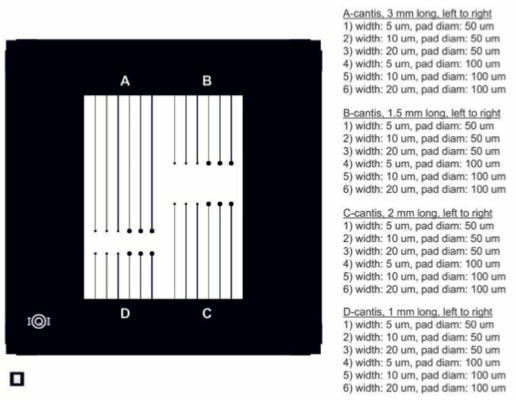
\includegraphics[scale=1]{../figures/cantilever.png}
	\caption{Multiple cantilever on one chip \cite{physikwiki}[p. 6]}
	\label{fig:cantilever}
\end{figure}
\subsection{Dampend driven harmonic oscilliation}
With a pulsed laser and a previous described cantilever we can build a oscillator that responds to the force of the photons. Because we want to measure a very tiny pressure the cantilever has to be driven by the pulsed laser at the resonance frequency of the oscillator. Due to the fact that we don't cool or evacuate our setup we have a dampening that is overcome by the repeated pulsing of the laser with the resonance frequency.\\
The calculation of the (mechanical) oscillator is stated in the experimental description \cite{physikwiki}.\\
Properties of the oscillator are the resonance frequency and the quality factor (taken from \cite{physikwiki}[p. 3-4]).\\
The quality factor:
$$Q = \frac{\omega_{0}}{\gamma}$$
Resonanz frequency :
$$\omega_0 = \sqrt{\frac{k}{m}}$$

%%%%%%%%%%%%%%%%%%%%%%%%%%%%%%%%%%%%%%%%%%%%%%%%
%%%%%%%%%%%%%%%%%%%%%%%%%%%%%%%%%%%%%%%%%%%%%%%%
\section{Experimental assembly}
We have a build up table top experiment composed of different components which can be seen in \ref{fig:setup}. The used cantilevers were the ones seen in \ref{fig:cantilever} denoted by D and one on A.\\
\begin{figure}[H]
	\centering
	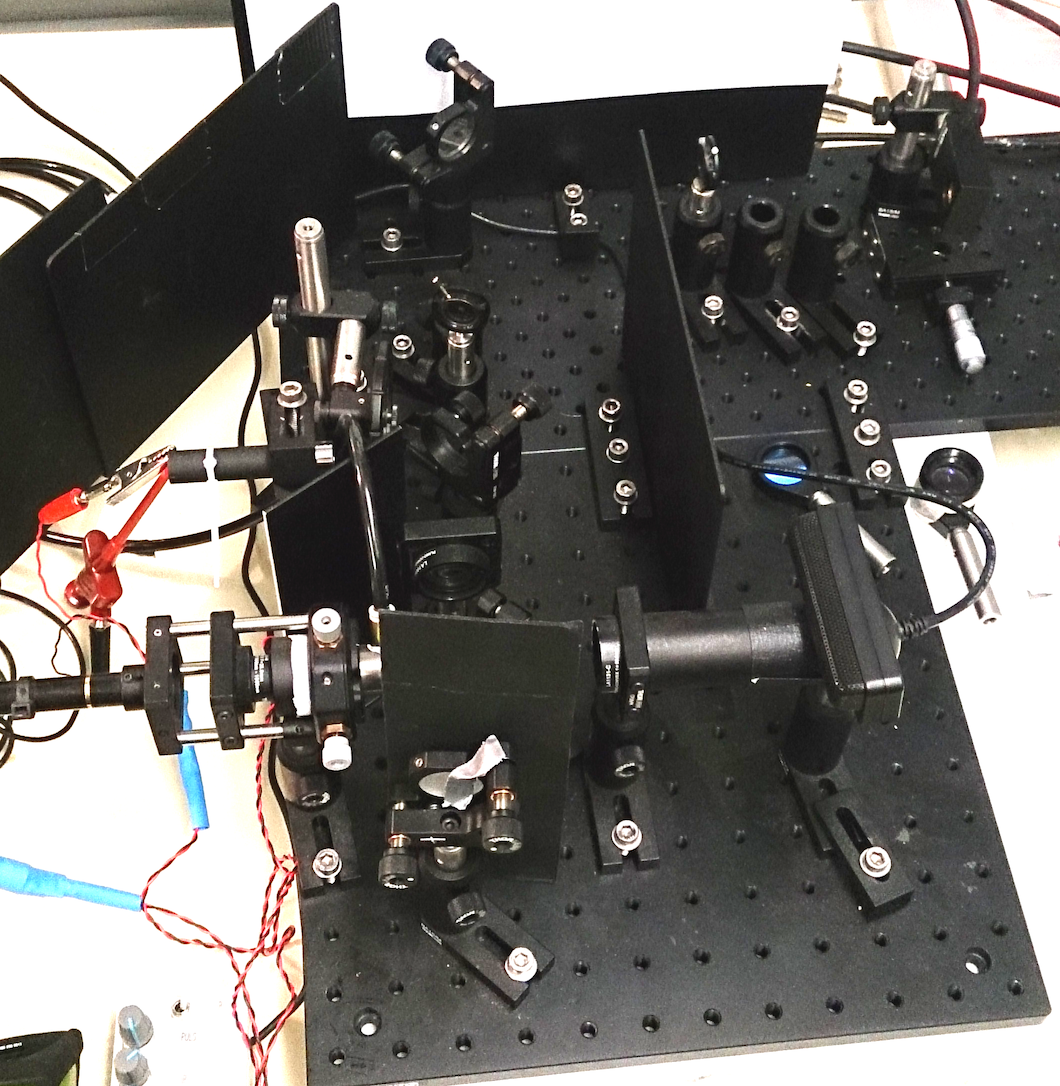
\includegraphics[scale=0.2]{../figures/aufbau.png}
	\caption{Setup}
	\label{fig:setup}
\end{figure}

\noindent
\textbf{Parts of the experiment}
\begin{itemize}
	\item Pulsed red laser 1064nm approximatly 2mW (left side figure \ref{fig:setup})
	\item Green laser 532nm build to interferometer (middle figure \ref{fig:setup})
	\item Beamsplitter to split the green beam (center figure \ref{fig:setup})
	\item PS3 cam for laser alignment (right side \ref{fig:setup})
	\item Quadropol photo diode (sensor) for displacement measurement by 4 photodiodes separated by a tiny gap (right upper figure \ref{fig:setup})
	\item Speaker for acoustic drive 
	\item Mirrors and lenses to modify the way of the laser
	\item Paper pieces and protection glasses as the experimentalist's best friends
	\item Oscilloscope to handle trigger and measure power aswel as displacement (figure \ref{fig:measurement})
\end{itemize}


\textbf{Summary of approach}\\
We have a chip (figure \ref{fig:cantilever} ) with different cantilever on it. A green laser built into a interferometer is used to observe the motion of the cantilever. Measuring the displacement is done with a quadrant photodiode (sensor). We determine the resonance frequency of different cantilever using acoustic drive by a speaker. This is done be search for the resonance frequency from 500Hz to 3.5kHz. With a PS3 camera the cantilever is focused by the green laser and from the other side from the pulsed red laser. We determine a resonance curve for one cantilever and protocol the phase and normalize the amplitude. Then we calculate the proportional constant (V/m) to get a displacement in meter on the sensor. After focusing both lasers on the cantilever and triggering the pulsed laser on the resonance frequency of the cantilever we can calculate the quality factor, the spring constant using the force of the laser (power-meter) and the full-width half maximum ($\gamma$ factor) of the resonance curve.

\begin{figure}[H]
	\centering
	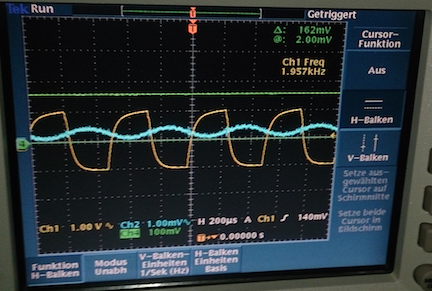
\includegraphics[scale=0.5]{../figures/messung.png}
	\caption{Measurement of data. Yellow:  Trigger for pulsed laser or acoustic drive. Cyan: Response on the sensor. Green: Interferometer power.}
	\label{fig:measurement}
\end{figure}

\noindent
\textbf{How to interpret the measurement}\\
Now combine the theory from \ref{theory} into one formula with the knowledge about the oscillator in \cite{physikwiki}:
$$\gamma = \frac{D}{m} = \frac{\omega_0}{Q}$$
From the solution to the harmonic driven dampened oscillator in \cite{physikwiki} we derive a formula for the position:
$$x_0 = \frac{F_0}{m}  \frac{1}{\sqrt{ (\omega_0^2 - \omega^2 )^2 + \gamma^2  \omega^2}}$$
Because the interesting point is where $\omega_0 = \omega$ (resonance) we can set that to zero and get
$$x_0 = \frac{F_0}{m} * \frac{1}{\gamma  \omega}$$
using the definition for $\gamma$ and $\omega_0^2$ we get
$$k = \frac{F_0 * Q}{x_0}$$
for the spring constant.\\
The $x_0$ is what we measure depending on the intensity of the laser, the displacement on the sensor (figure \ref{fig:sensorsensitivity}), the distance of the beam from cantilever to sensor and the length of the cantilever (resulting in a conversion factor from sensor result to displacement). The length of the cantilever itself was also used but with length one does not contribute much more than it's unit.\\

The interferometer is aligned that with no (or tiny) motion of the cantilever it is possible to see interference of the two rays on the wall. When the cantilever oscillates there is a phase shift which leads to destructive interference and the pattern disappears. This can be seen in figure \ref{fig:pattern}.

\begin{figure}[H]
	\centering
	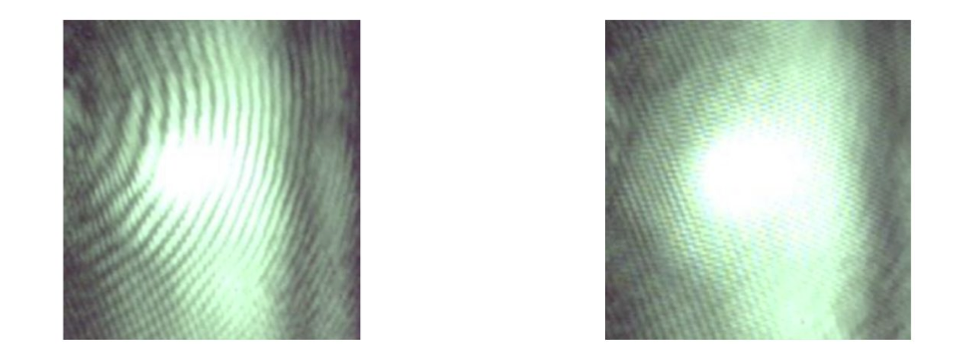
\includegraphics[scale=0.6]{../figures/interference.png}
	\caption{Left: Interference pattern without driving. Right: Destructive interference with drive \cite{physikwiki}[p. 9, figure 5]}
	\label{fig:pattern}
\end{figure}
%%%%%%%%%%%%%%%%%%%%%%%%%%%%%%%%%%%%%%%%%%%%%%%%
%%%%%%%%%%%%%%%%%%%%%%%%%%%%%%%%%%%%%%%%%%%%%%%%
\section{Results}
The full document and the results contained in a QTI file and a Excel sheet can be found under \cite{github}.

\begin{figure}[H]
 \centering
 \pgfplotstabletypeset[
 columns={cantilever, omega},
 col sep=&,
 columns/cantilever/.style={string type, column name=\makecell{$Name$\\ from \ref{fig:cantilever}} },
 columns/omega/.style={column name=\makecell{$\omega_{res}$ \\ ($\pm$ 10)[Hz]}, precision=0},
 every head row/.style={before row=\hline,after row=\hline\hline},
 every last row/.style={after row=\hline},
 every first column/.style={column type/.add={|}{} },
 every last column/.style={column type/.add={}{|} }
 ]{
 cantilever & omega
 A6 & 680
 D4 & 1870 
 D5 & 2565 
 D6 & 3395
 }
 \caption{Resonance frequency of four cantilever (acoustic driven)}
 \label{tab:acoustic_resonance}
\end{figure}

\noindent
\textbf{From now on we focus on the cantilever D4}\\
As described in the theory part we calculated a conversion constant as follows:
$$C = (7.2 \pm 0.8) \frac{1}{mm}$$
We have 1 per mm because the error resulting from intensity fluctuations was compensated through normalizing the amplitude by the power of the laser at the time of the measurement. Because the laser intensity range goes from 80mV to 290mV (figure \ref{fig:resonanzkurvedata} "LaserCountSum") we have a huge error as seen below.\\
The length of the green laser from the cantilever to the sensor was also needed to calculate the constant:
$$L = (57.3 \pm 2)cm$$
At last we need the intensity of the green laser which was about 
$$I_{green} = (185 \pm 100)mV$$
We measured the resonance curve for the cantilever as seen in figure \ref{fig:resonanzkurve}.
With this we could read out the full-width half maximum value which is the value of the $\gamma$ factor in the calculation.\\
The resulting quality factor is
$$Q = 31.694$$
The length of the cantilever is 1mm.

\begin{figure}[H]
	\centering
	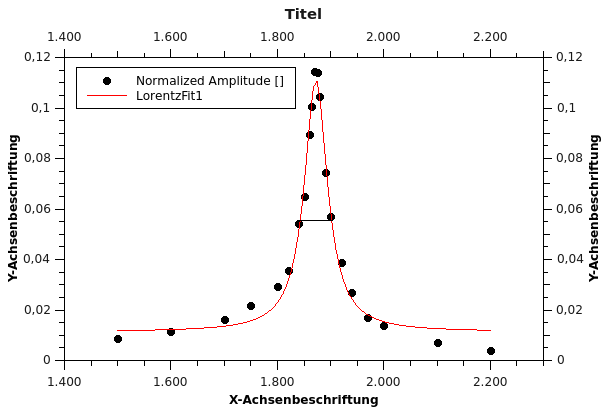
\includegraphics[scale=0.4]{../figures/Resonanzkurve.png}
	\caption{Resonance curve with Lorentz fit of D6}
	\label{fig:resonanzkurve}
\end{figure}

\begin{figure}[H]
	\centering
	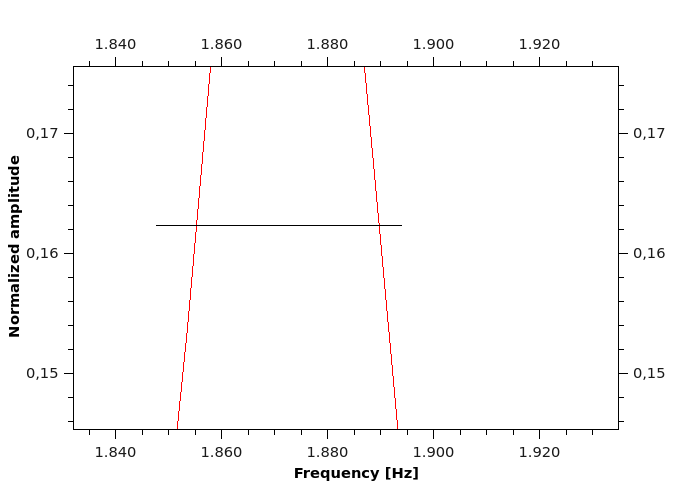
\includegraphics[scale=0.4]{../figures/ResonanzkurveHalbwertsbreite.png}
	\caption{Full width half maximum of the resonance curve D6}
	\label{fig:resonanzkurvehmfuw}
\end{figure}

\end{multicols}
\begin{figure}[H]
	\centering
	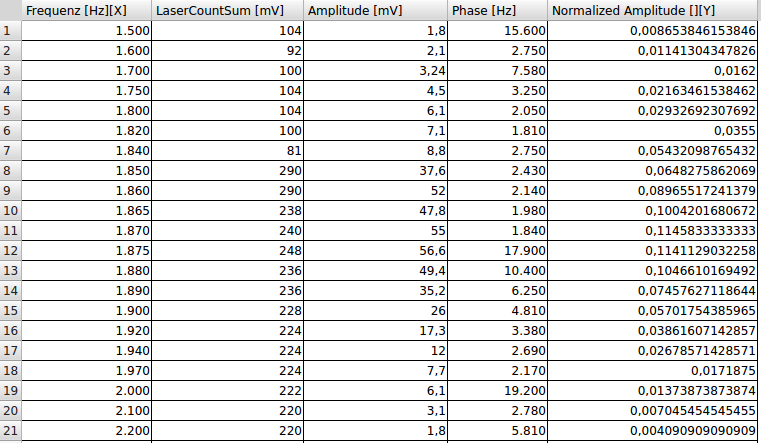
\includegraphics[scale=0.5]{../figures/rohdaten.png}
	\caption{Raw data on observed cantilever D6}
	\label{fig:resonanzkurvedata}
\end{figure}
\begin{multicols}{2}

\begin{figure}[H]
	\centering
	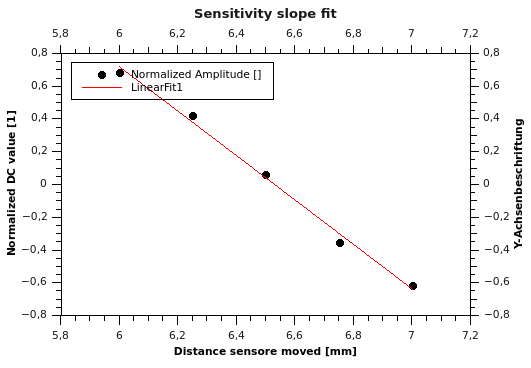
\includegraphics[scale=1.4]{../figures/Slopeofsensitivityofthesensor.png}
	\caption{Slope of the sensitivity of the quadrant sensor used to obtain the proportion constant C}
	\label{fig:sensorsensitivity}
\end{figure}

For the laser driven oscillation we get:
$$k = (29 \pm 1) [\frac{mN}{m}]$$
$$x = (11 \pm 0.5) nm$$
with a power of the driving laser of 1.5mW.


%%%%%%%%%%%%%%%%%%%%%%%%%%%%%%%%%%%%%%%%%%%%%%%%
%%%%%%%%%%%%%%%%%%%%%%%%%%%%%%%%%%%%%%%%%%%%%%%%
\section{Discussion}
For a experiment at room temperature with normal air pressure and costs below \EUR{1000} one can learn and see a lot. \\
The alignment process was done fast because the setup of the interferometer was already done. Getting the green and red laser on the cantilever was intuitive using the image of the PS3 camera. \\
The acoustic driven measurements where annoying because the frequency for the 1mm cantilever had to be in the area of 1-3.5kHz which is a awful noise.\\
The result of some nanometer displacement is in the area of what we were expecting of a 1mm cantilever. Problematic was the right use of the green laser because of the high fluctuations between measurements. Because of that we increased the error that was calculated. Another reason is that about 300$\mu V$ were already background radiation.\\
Answering the optional question if we could make the determination of the physical displacement read out with the interferometer better:\\
No, with a displacement of about 10nm there seems to be no way to be more accurate. It is a really good experiment to learn how to work with lenses, iris, sensor and other optical equipment. The reason is that it is a simple setup with not many elements to adjust.

%%%%%%%%%%%%%%%%%%%%%%%%%%%%%%%%%%%%%%%%%%%%%%%%
%%%%%%%%%%%%%%%%%%%%%%%%%%%%%%%%%%%%%%%%%%%%%%%%

\bibliography{protocol.bib}
\bibliographystyle{plain}

\end{multicols}
\end{document}